\documentclass[12pt]{article}
\usepackage{amsmath,setspace,graphicx,amssymb,amsthm,float}
\usepackage{hyperref}
\hypersetup{
    colorlinks,
    allcolors=black
}
\title{\textbf{MATH2104 Methods for Differential Equations Lecture Notes}}
\author{Thomas Piercy}
\date{\today{}}
\setcounter{section}{-1}

\newcommand{\df}[2]{\frac{\text{d}#1}{\text{d}#2}}
\newcommand{\seq}[2]{(#1_#2)_{#2\in\mathbb{N}}}
\newcommand{\pf}[2]{\frac{\partial #1}{\partial #2}}
\begin{document}
\maketitle
\hrulefill
\tableofcontents
\newpage
\setstretch{1.5}
\section{Key Module Information}
\begin{itemize}
    \item The exam questions in this module are often inspired by the questions in the additional reading section of the module syllabus. They are also taken from the problem sheets (sometimes without alteration).
    \item This module will be heavily affected by strike action, so use the full lecture notes to keep up to date.
    \item On the problem sheets, difficulty 2 questions are the same difficulty and detail as exam questions. Difficulty 3 questions are for further understanding of the material.
\end{itemize}
\section{Introduction to 2\textsuperscript{nd} Order ODEs}
\subsection{Background}
A differential equation (DE) is an equation involving derivatives. For example:
\begin{align*}
    &y''(x)+y(x)=0 && \text{(ODE)}\\
    &\pf{u}{t}+\pf{u}{x}=0 && \text{(PDE)} \\
    &u_t+u_x=0 && \text{(PDE)}
\end{align*}
The order of a DE is the highest derivative. This tells you the style and method for solving the equation.
\begin{align*}
    u_t=u_{xx} && \text{(2nd order PDE)}
\end{align*}
A DE is linear if the dependant variable and its derivatives only appear in a linear fashion. For example, Airy's equation:
\[y''-xy=0\]
Is linear. Most of this module only deals with linear ODEs. A DE is homogeneous if all terms in the DE involve the dependant variable (and/or its derivatives). Otherwise it is inhomogeneous.
\begin{align*}
    &y''+y=xy' && \text{homogeneous} \\
    &u_{tt}=u_{xx}+e^{-t} && \text{inhomogeneous}
\end{align*}
Homogeneity also determines the method used to solve the DE.
\subsection{First Order ODEs}
First order ODEs are of the form:
\[y'(x)=f(x,y)\]
The form of \(f(x,y)\) gives us the solution methods:
\begin{itemize}
    \item Separable: \(f(x,y)=g(x)h(y)\), solve via integration.
    \item Linear:
    \begin{enumerate}
        \item Transform into canonical form: \(y'+p(x)y=q(x)\).
        \item Calculate integrating factor: \(r(x)=\exp(\int p(x)\,\text{d}x)\)
        \item Multiply canonical ODE by integrating factor.
        \item Notice that \((yr)'=y'\cdot r+y\cdot r\cdot p(x)\).
        \item \([y(x)r(x)]'=q(x)r(x)\)
        \item \(y(x)r(x)=\int q(x)r(x)\,\text{d}x\;+c\)
    \end{enumerate}
\end{itemize}
\subsubsection*{Example}
\[xy'-y=x^2\sin{x}\]
\[y'-\frac{1}{x}=x\sin{x}\]
\[r(x)=\exp{\left(\int -\frac{1}{x}\,\text{d}x\right)}\]
\[r(x)=x^{-1}\]
\[\left(\frac{y}{x}\right)'=\sin{x}\]
\[\frac{1}{x}y=-\cos{x}+c\]
\[y=x(c-\cos{x})\]
\subsection{Second Order Linear ODEs}
These equations have canonical form:
\[y''+p(x)y'+q(x)y=r(x)\]
There is no general method for solving 2nd order linear ODEs but we do know that a general solution would be compromised of two terms: A homogeneous component and a particular solution.
\[y_g(x)=y_h(x)+Y(x)\]
Where \(y_h(x)\) satisfies: \(y_h''+p(x)y_h'+q(x)y_h=0\) and we can express \(y_h\) in the form:
\[y_h=Ay_1(x)+By_2(x)\]
We can do this because of the linearity. What this means is that given two solutions that are "distinct enough" we can generate the entire class of solutions. Formally, "distinct enough" requires that the two solutions be linearly independent:
\[c_1y_1(x)+c_2y_2(x)=0\iff c_1,c_2=0\]
Linear independence also means that \(y_h\equiv 0\) is never included as one of the distinct solutions to the equation (since this gives us no information anyway).
\subsubsection{The Wronskian}
The Wronskian, \(W(y_1,y_2)\) in 2D, is defined as:
\[W(x)=W(y_1,y_2)=\det\begin{pmatrix}
    y_1(x) & y_2(x) \\
    y_1'(x) & y_2'(x)
\end{pmatrix}\]
Notice that the order of the solutions does matter generally. It is important to remember which solution is which. If the Wronskian is non-zero, then the two solutions are linearly independant at a given point.
\subsubsection{Analytic Functions (Applied Def)}
A function \(f(x)\) is analytic at \(x=x_0\) if it can be expressed as a Taylor series at \(x=x_0\):
\[f(x)=\sum^\infty_{n=0}a_n\cdot(x-x_0)^n\]
Where:
\[a_n=\frac{1}{n!}\cdot\lim_{x\to x_0}\df{^nf}{x^n}\]
Some key examples to remember are:
\begin{itemize}
    \item Exponential, sinusoidal, and polynomial functions are analytic everywhere.
    \item Irreducible rational functions are analytic everywhere except at roots (to avoid division by 0).
    \item The rational functions \(x^q,\ q\notin \mathbb{N}\cup \{0\}\) are analytic for all \(x>0\) but not for \(x=0\). Similarly \(x^q\log(x)\) has this property.
    \item Addition, multiplication, and composition of analytic functions is also analytic. It is possible (but not guaranteed) that analytic and non-analytic functions can combine to an analytic function. e.g \(\sin(x)/x\).
\end{itemize}
\subsubsection{Existence and Uniqueness}
Consider a DE in canonical form:
\[y''+p(x)y'+q(x)y=r(x)\]
If \(p(x),\, q(x),\, r(x)\) are all analytic at \(x=x_0\), then there exists a unique solution \(y(x)\) satisfying the initial conditions:
\begin{align*}
    &y(x_0)=a \\
    &y'(x_0)=b
\end{align*}
For example:
\[x^2y''+4xy'+2y=0\]
Can not satisfy any initial conditions at \(x=0\), since \(p(x)=4/x\) is not analytic at \(x=0\). We can know this without even having to solve the equation, which can be very useful when dealing with complex ODEs. That isn't to say that the ODE doesn't have a general solution - it very well might. It is just that the general solution cannot also solve an IVP at certain points if non-analytical.
\subsubsection{Fundamental set of solutions}
Consider the equation:
\[y''(x)+p(x)y'(x)+q(x)y=0\]
The fundamental set of solutions links the initial conditions \(y(x_0)=A,\ y'(x_0)=B\) to the guaranteed two solutions \(y_1(x)\) and \(y_2(x)\). The FSS have the property that:
\begin{align*}
    &y_1(x_0)=1 & y_1'(x_0)=0 \\
    &y_2(x_0)=0 & y_2'(x_0)=1
\end{align*}
Notice that this forces the Wronskian into an identity matrix. In particular this maps the IVP solution to the above equation:
\[y(x)=Ay_1(x)+By_2(x)\]
However note that this only applies to initial condition problems and not boundary condition problems which have their own set of methods for solving.
\subsection{Solving constant-coefficient homogeneous 2nd order ODEs}
Exactly the same as in Year 1, we take the equation:
\[y''+p(x)y'+q(x)y=0\]
With:
\[p(x)=\frac{b}{a},\ q(x)=\frac{c}{a}\]
Then:
\[ay''+by'+c=0\]
We use the ansatz \(y=e^{rx}\) where \(r\) is some constant. After substitution this leave us with:
\[e^{rx}(ar^2+br+c)=0\]
Which in turn forces the bracket to be \(0\) and this is known as our auxiliary equation. We have \(r_+\) and \(r_-\) from solving the quadratic equation although we might find it easier  to leave in the form \(r=\alpha+\beta\) where \(\alpha=\frac{-b}{2a}\) and \(\beta=\frac{\sqrt{b^2-4ac}}{2a}\).
\subsubsection*{Case 1: \(\Delta>0\)}
Here we have \(r_{\pm}\in\mathbb{R}\) and \(r_+\ne r_-\). We are left with the general solution:
\[y(x)=Ae^{r_+x}+Be^{r_-x}=e^{\alpha x}[C\sinh{(\beta x)}+D\cosh{(\beta x)}]\]
\subsubsection*{Case 2: \(\Delta=0\implies\beta=0\)}
\[y(x)=Ae^{\alpha x}+Bxe^{\alpha x}\]
\subsubsection*{Case 3: \(\Delta<0\implies\beta=i\gamma\)}
\[y(x)=e^{\alpha x}[Ae^{i\gamma x}+Be^{-i\gamma x}]=e^{\alpha x}[C\sin{(\gamma x)}+D\cos{(\gamma x)}]\]
\subsection{Change of Variables}
The idea behind a change of variables is that we compute \(y(x)\) via an intermediary \(u(w(x))=u(w)\), where \(w\) is a given function. To perform the change, we need to know some derivatives and we can get these from chain and product rule applications. In the below working, a dotted derivative means a derivative with respect to \(w\) and a primed derivative means a derivative with respect to \(x\):
\[\df{u}{x}=\df{u}{w}\df{w}{x}=\dot{u}\cdot w'(x)\]
\[\df{^2u}{x^2}=\df{}{x}\left(\df{u}{x}\right)=\df{}{x}(\dot{u})w'(x)+\dot{u}w''(x)\]
\[=\ddot{u}\cdot (w'(x))^2+\dot{u}\cdot w''(x)\]
You need to memorise these equations, they are vital to the change of variables method and this module. When performing the change of variables, essentially just substitute \(y\) with \(u\) and the derivatives we calculated. This turns the ODE into another ODE in terms of \(u\).
\subsubsection*{Example}
Using \(w=x^2\), solve \(xy''(x)-y'(x)+4x^3y=0\).
\begin{align*}
    &w'(x)=2x \\
    &w''(x)=2
\end{align*}
\[x\cdot[4x^2\cdot\ddot{u}+2\dot{u}]-[2x\cdot\dot{u}]+4x^3u=0\]
This simplifies down to:
\[4x^3(\ddot{u}+u)=0\]
But since we want our solution to be valid for all \(x\), we are required to make the bracket \(0\). This is just solving a new ODE in terms of \(u\). Then:
\[u(w)=C\sin(w)+D\cos(w)\implies y=C\sin(x^2)+D\cos(x^2)\]
\subsection{Euler Equations}
The next best thing after constant-coefficient ODEs are Euler equations. These also provide an auxiliary equation following an ansatz but it is different to the constant coefficient case. We need to be careful to state both our auxiliary equation and our ansatz that got us there in an exam. An Euler equation takes the form:
\[ax^2y''(x)+bxy'(x)+cy=0\]
with \(a,b,c\in\mathbb{R}\). Our ansatz is:
\begin{align*}
    &y=x^r \\
    &y'=rx^{r-1} \\
    &y''=r(r-1)x^{r-2}
\end{align*}
Substituting in gets us:
\[x^r[ar(r-1)+br+c]=0\]
Notice that the auxiliary equation is still a quadratic, but it is a different quadratic to before. Once again we have solutions of the form \(r=\alpha+\beta\) with:
\begin{align*}
    &\alpha=\frac{a-b}{2a}, & \beta=\frac{\sqrt{(b-a)^2-4ac}}{2a}
\end{align*}
Because we use the discriminant quite a lot, we can shorthand it to \(\Delta\).
\subsubsection*{Case 1: \(\Delta>0\)}
\[y(x)=Ax^{r_+}+Bx^{r_-}\]
\subsubsection*{Case 2: \(\Delta=0\)}
\[y(x)=x^r[A+B\log{x}]\]
\subsubsection*{Case 3: \(\Delta<0\implies \beta=i\gamma\)}
\[y(x)=x^\alpha[Ax^{i\gamma}+Bx^{-i\gamma}]=x^{\alpha}[A\sin{(\gamma\log x)+B\cos{(\gamma \log x)}}]\]
Notice that the change of variables \(w=\log x\) is sufficient to turn an Euler equation into a constant-coefficient ODE.
\subsection{Reduction of Order}
Given one solution, \(y_1(x)\) that solves:
\[y''+p(x)y'+q(x)y=0\]
We ca find a second linearly independent solution:
\[y_2(x)=u(x)\cdot y_1(x)\]
Substituting this into our original ODE gives us:
\[y''_1u+2y_1'u'+y_1u''+p(x)[y_1'u+y_1u']+q(x)\cdot y_1u=0\]
\[\implies y_1u''+u'[2y_1'+p(x)y_1]+u[y''_1+p(x)y'_1+qy_1]=0\]
Notice how we have a copy of our original ODE in canonical form, except with the function \(y_1(x)\). We know this function solves the ODE so we can substitute the right-hand side into our expression to clean it up.
\[y_1u''+u'[2y_1'+p(x)y_1]=0\]
Let \(v=u'\).
\[y_1v'+v[2y_1'+p(x)y_1]=0\]
Now notice that we have reduced the equation to a first order ODE. We need this ODE to be in canonical form and then we can use the integrating factor method to solve it.
\[v'+v\left[\frac{2y_1'}{y_1}+p(x)\right]\]
\begin{align*}
    r(x)&=\exp\left(\int\frac{2y_1'}{y_1}+p(x)\,\text{d}x\right) \\
    &=\exp\left(2\int\frac{y_1'}{y_1}\,\text{d}x+\int p(x)\,\text{d}x\right) \\
    &=\exp\left(2\log(y_1)+\int p(x)\,\text{d}x\right) \\
    &= y_1^2\exp\left(\int p(x)\,\text{d}x\right)
\end{align*}
Then multiplying through and integrating gets us:
\[v(x)=u'(x)=\frac{C}{r(x)}=\frac{C}{y_1^2}\left(-\int p(x)\,\text{d}x\right)\]
And now we have an explicit formula for \(u'(x)\) which means that integrating this gets us our helper function \(u(x)\) which allows us to work out the second solution.
\[y_2(x)=u(x)\cdot y_1(x)\]
\subsubsection*{Example, Euler equation}
Consider the Euler equation:
\[x^2y''+x(1-2m)y'+m^2y=0\]
We use the \(x^r\) ansatz which leaves us with:
\[r(r-1)+r(1-2m)+m^2=0\implies r=m\]
So we have \(y_1(x)=x^m\). We can use reduction of order to find the second solution: Let \(y_2(x)=u(x)\cdot y_1(x)\).
\[u'(x)=\frac{C}{x^{2m}}\exp{\left(-\int \frac{1-2m}{x}\,\text{d} x\right)}\]
\[u'(x)=\frac{C}{x^{2m}}\exp((2m-1)\log(x))\]
\[u'(x)=\frac{C}{x^{2m}}x^{2m-1}=\frac{C}{x}\]
\[u'(x)=\frac{C}{x}\implies u(x)=C\log x\]
Then \(y_2(x)=C\cdot x^m\log(x)\). Note that we do not need to introduce a second constant of integration here due to linearity.
\subsection{Variation of Parameters}
You may be wondering how to deal with inhomogeneous ODEs. For the ODE in canonical form:
\[y''+p(x)y'+q(x)y=r(x)\]
and given \(y_1(x), y_2(x)\) we can solve for a single particular solution that satisfies the inhomogeneity.
\[Y(x)=u_1(x)y_1(x)+u_2(x)y_2(x)\]
Using the general product rule we get:
\begin{align*}
    &[u_1''y_1+2u_1'y_1'+u_1y_1''+u_2''y_2+2u_2'y_2'+u_2y_2'']\\
    &+p(x)[u_1'y_1+u_1y_1'+u_2'y_2+u_2y_2']\\
    &+ q(x)[u_1y_1+u_2y_2]\\
    &=r(x)
\end{align*}
This simplifies down to something also quite long and horrible but what is key is that we have one equation of two unknowns. Whilst in this undetermined form and with us being able to freely choose \(u_1\) and \(u_2\) we can impose our own additional condition to make the ODE easier to solve. In most cases we set:
\[u_1'y_1+u_2'y_2=0\]
so to remove the \(q(x)\) term in the ODE. This equation also provides us the differential equation:
\[(u_1'y_1+u_2'y_2)'=0\]
Which allows us to simplify our long and horrible ODE into a set of linear equations.
\[\begin{cases}
    u_1'y_1'+u_2'y_2'=r(x) \\
    u_1'y_1+u_2'y_2=0
\end{cases}\]
Solving this system gives us:
\[u'_1(x)[y_1y_2'-y_1'y_2]=-y_2(x)r(x)\]
\[\implies u_1=-\int\frac{y_2(x)r(x)}{W(y_1,y_2)}\,\text{d}x\]
Similarly we can work out \(u_2\). Finally we can substitute these functions back in to our definition of the particular solution \(Y(x)\) and we get:
\[Y(x)=-y_1(x)\left[\int\frac{y_2(x)r(x)}{W(y_1,y_2)}\,\text{d}x\right]+y_2(x)\left[\int\frac{y_1(x)r(x)}{W(y_1,y_2)}\,\text{d}x\right]\]
This, mercifully, is on the formula sheet.
\clearpage
\section{Series Solutions}
Sometimes all of our other solution methods fail but we still want to examine the behaviour of ODE solutions close to an expansion point \(x_0\). Throughout this chapter we will focus on the ODE:
\[P(x)y''+Q(x)y'+R(x)y=0\]
\subsection{Ordinary and Singular Points}
For the above ODE, a point \(x_0\in\mathbb{C}\) is called an ordinary point if the functions \(Q(x)/P(x)\) and \(R(x)/P(x)\) are both analytic at \(x=x_0\). Otherwise \(x=x_0\) is a singular point. This definition can be cumbersome to use so for the purposes of this module we will use a looser definition. For the standard ODE we are dealing with in this module, a point \(x_0\in\mathbb{C}\) is called an ordinary point if:
\begin{align*}
  &\lim_{x\to x_0}\frac{Q(x)}{P(x)} \\
  &\lim_{x\to x_0}\frac{R(x)}{P(x)}
\end{align*}
both exist. Otherwise we say \(x_0\) is a singular point. Furthermore if our the canonical form contains functions of \(\log(z)\) or \(z^q,\ q\ne\mathbb{N}\cup 0\), then \(x_0\) is singular. Note that this definition is certainly not true in general but suffices for this module.
\subsubsection*{Example}
\[y''+\log (x-2)y'+\sqrt{x^2+4}y=0\]
\begin{align*}
    &P(x)=1 \\
    &Q(x)=\log(x-2) \\
    &R(x)=\sqrt{x^2+4}
\end{align*}
Notice that \(Q(x)\) fails to be analytic when \(x=2\) and \(\sqrt{x^2+4}\) fails when \(x=\pm 2i\). This means the singular points are \(x_0=2,\pm 2i\).
\subsection{Series Ansatz Formulation}
For an ODE of the form:
\[P(x)y''+Q(x)y'+R(x)y=0\]
We have, by definition, that the functions in it's canonical form can be expressed as a Taylor series expanded about \(x=x_0\):
\begin{align*}
    &\frac{Q(x)}{P(x)}=\alpha_0+\alpha_1(x-x_0)+\dots \\
    &\frac{R(x)}{P(x)}=\beta_0+\beta_1(x-x_0)+\dots
\end{align*}
Then close to \(x_0\) we can approximate the ODE as:
\[y''+\alpha_0y'+\beta_0y+\cdots=0\]
Which is a constant-coefficient ODE. We can then expect the solution \(y(x)\) to be analytic near \(x=x_0\) and so can be represented with a Taylor series:
\[y(x)=\sum^\infty_{n=0}a_n(x-x_0)^n\]
Then we can calculate the derivatives of this ansatz and substitute into the ODE. We then need to compare coefficients to find a recurrence relation.
\subsubsection{Worked Example}
We wish to consider the following ODE:
\[(x^2+1)y''+y=0\]
near to the point \(x=x_0\). \(x=x_0\) is an ordinary point so we can use the series expansion.
\begin{align*}
    &y(x)=\sum^\infty_{n=0}a_nx^n \\
    &y'(x)=\sum^\infty_{n=0}na_nx^{n-1} \\
    &y''(x)=\sum^\infty_{n=0}n(n-1)a_nx^{n-2}
\end{align*}
Substituting into the ODE we get:
\[\sum^\infty_{n=0}x^2a_nn(n-1)x^{n-2}+\sum^\infty_{n=0}n(n-1)a_nx^{n-2}+\sum^\infty_{n=0}a_nx^n=0\]
We need to shift the indices so that all of our monomials have the same power:
\[\sum^\infty_{n=-2}(n+2)(n+1)a_{n+2}x^{n}\]
We then need to move the first two terms to get back to the right starting index. We can then combine all of the summations:
\[\sum^\infty_{n=0}x^n[(n+2)(n+1)a_{n+2}+(n(n-1)+1)a_n]=0\]
We can then compare coefficients to get the following recurrence relation:
\[a_{n+2}=-\frac{n^2-n+1}{(n+2)(n+1)},\quad n\geq 0\]
Some recurrence relations are explicitly solvable whereas others we have to compute numerically. Since the relation holds for \(n\geq 0\), the first coefficient we can compute is \(a_{2}\). Then \(a_0\) and \(a_1\) are left to choose freely. We know a fundamental set of solutions exists due to the conditions of an ordinary point. Note that:
\[y(0)=a_0\qquad y'(0)=a_1\]
We can then find our two linearly independent solutions by first setting \(a_0=0\) with \(a_1\) free, and then setting \(a_1=0\) with \(a_0\) being free.
\[y_1(x)=a_0\left[1-\frac{x^2}{2}+\frac{x^4}{8}+\cdots\right]\]
\[y_2(x)=a_1\left[x-\frac{x^3}{6}+\frac{7x^5}{120}+\cdots\right]\]
Note that sometimes \(y_1\) or \(y_2\) will either be a known infinite series or will be finite - implying the solution is a polynomial.
\subsubsection*{Example}
\[(x^2+1)y''+xy'-y=0,\quad x_0=0\]
\[\lim_{x_0\to 0}\frac{x}{x^2+1}=0\]
The limit exists so \(x_0\) is an ordinary point. We can construct a series ansatz:
\[y(x)=\sum^\infty_{n=0}a_nx^n\]
\[\sum^\infty_{n=0}n(n-1)a_nx^n+\sum^\infty_{n=0}n(n-1)a_nx^{n-2}+\sum^\infty_{n=0}na_nx^n-\sum^\infty_{n=0}a_nx^n=0\]
\[\implies n(n-1)a_n+(n+2)(n+1)a_{n+2}+na_n-a_n=0\]
\[\implies a_{n+2}=\frac{(1-n)a_n}{n+2},\quad n\geq 0\]
Set \(a_1=0\) and let \(a_0\) be free. Then:
\[a_2=\frac{a_0}{2}\implies a_4=-\frac{a_0}{8}\]
\[a_{2n+1}=0\]
\[\implies y_1(x)=a_0+\frac{x^2}2{a_0-\frac{x^4}{8}a_0+\cdots}\]
Now set \(a_0=0\) and \(a_1\) free. Then \(a_{2n}=0\) which means that our choice for \(a_1\) solves the ODE in a polynomial way. We choose the simplest solution: \(a_1=1\). Then:
\[y_2(x)=x\]
\[y(x)=a_0\left[1+\frac{x^2}{2}-\frac{x^4}{8}+\cdots\right]+a_1x\]
Notice that once we know a polynomial that explicitly solves the ODE, we can apply reduction of order to calculate the other one fully.
\subsection{Minimum Radius of Convergence}
As seen with series solutions expanded about ordinary points, we can (in theory), keep adding more and more terms to our series solution to improve the approximation of the true ODE solution near its expansion point. However, like a Taylor series, the functions local behaviour doesn't tell us anything about the global behaviour: notably we need to know what values our series solution agrees with the true ODE solution. For the ODE:
\[p(x)y''+q(x)y'+r(x)y=0\]
Its series solution expanded about the ordinary point \(x=x_0\) will converge to the true ODE solution on the domain \(|x-x_0|<R\), where \(R\) is the smallest distance in \(\mathbb{C}\) between \(x_0\) and any singular points \(x_s\) of the ODE.
\[R=\min_{x_s}|x_0-x_s|\]
The value \(R\) is known as the minimum radius of convergence.
\subsubsection*{Examples}
The minimum radius of convergence for the ODE:
\[(x^2+1)y''+xy'-y=0,\quad x_0=0\]
is calculated based on the singular points \(x=\pm i\). We have:
\[R=|0-i|=|0+i|=1\]
Hence the series solutions are only guaranteed to agree with the ODE solutions for \(|x|<1\). Note that the minimum radius of convergence \(R\) not only depends on the location of the singular points \(x_s\in\mathbb{C}\) but also on the expansion point \(x_0\).
\subsection{Series Solutions at a Regular Singular Point}
We have just looked at what we need to do if we want to expand around an ordinary point, and we have seen that we cannot use this method to expand around a singular point. However, expanding around a singular point is a valid mathematical concept and it may well be something we wish to do so we need a new technique to do so. We are still restricted to a specific kind of singular point, but we can at least do something.
\subsubsection{Definitions}
For the standard ODE we are looking at in this chapter, a singular point \(x_0\in\mathbb{C}\) is called regular if the functions:
\begin{align*}
    &\frac{Q(x)}{P(x)}(x-x_0) \\
    &\frac{R(x)}{P(x)}(x-x_0)^2
\end{align*}
are both analytic at \(x=x_0\). Otherwise it is called an irregular singular point. For the purposes of this module, we will once again look at a simpler definition. A point \(x_0\in\mathbb{C}\) is a regular singular point if the limits:
\begin{align*}
    &\lim_{x\to x_0}\frac{Q(x)}{P(x)}(x-x_0) \\
    &\lim_{x\to x_0}\frac{R(x)}{P(x)}(x-x_0)^2
\end{align*}
both exist. Likewise if we contain log functions or non natural powers we have \(z=0\) as an irregular singular point.
\subsubsection*{Examples}
Consider the ODE:
\[(x^2+1)y''+xy'-y=0\]
This has singular points at \(x=\pm i\) and we can classify those singular points as above:
\begin{align*}
    &\lim_{x\to i}\frac{x(x-i)}{x^2+1}=\frac{1}{2} \\
    &\lim_{x\to i}\frac{-(x-i)^2}{x^2+1}=0
\end{align*}
Since both limits exist we say that \(x=i\) is a regular singular point. The same argument applies for \(x=-i\).
\subsection{The Frobenius Method}
In a similar way to ordinary point series solutions, we have:
\[\frac{Q(x)}{P(x)}(x-x_0)=\alpha_0+\alpha_1(x-x_0)+\cdots\]
\[\frac{R(x)}{P(x)}(x-x_0)^2=\beta_0+\beta_1(x-x_0)+\cdots\]
Where \(\alpha\) and \(\beta\) are well defined constants. This means we can approximate the ODE with:
\[(x-x_0)^2y''+\alpha_0(x-x_0)y'+\beta_0y+\cdots=0\]
Which is an Euler ODE!. Therefore we expect our solution to be approximated by:
\[(x-x_0)^r\]
Where \(r\) solves the auxiliary equation: \(r(r-1)^2+\alpha_0r+\beta_0=0\). Provided that the two solutions of \(r\) that solve this equation are real and distinct, we have our series solution should be modified by a factor of \((x-x_0)^r\). This is known as the Frobenius method. For the ODE:
\[P(x)y''+Q(x)y'+R(x)y=0\]
the series solution expanded around the singular point \(x=x_0\) will be of the form:
\[y(x)=(x-x_0)^r\sum^\infty_{n=0}a_n(x-x_0)^n\]
with two real and distinct solutions to \(r\) occurring via solving the auxiliary equation.
\subsubsection*{Example}
Consider the ODE:
\[4xy''+2y'+y=0\]
around the point \(x_0=0\). We have that \(x_0=0\) is a regular singular point by looking at limits. Because of this, we can use the Frobenius method:
\[y(x)=\sum^\infty_{n=0}a_nx^{n+r}\implies y'(x)=\sum^\infty_{n=0}(n+r)a_nx^{n+r-1}\]
\[\implies y''(x)=\sum^\infty_{n=0}(n+r)(n+r-1)a_nx^{n+r-2}\]
We can then substitute these terms into the ODE:
\[\sum^\infty_{n=0}4(n+r)(n+r-1)a_nx^{n+r-1}+\sum^\infty_{n=0}2(n+r)a_nx^{n+r-1}+\sum^\infty_{n=0}a_nx^{n+r}=0\]
Like before we need to match both monomial powers and starting indices:
\[\underbrace{\alpha_0x^{r-1}[4r(r-1)+2r]}_{n=-1}+\sum^\infty_{n=0}x^{n+r}\{[4(n+r)(n+r+1)+2(n+r+1)]a_{n+1}+a_n\}\]
Since each coefficient should be zero, we end up with two equations - one for \(r\) and one for the recurrence relation involving \(a_n\).
\begin{align*}
    &4r(r-1)+2r=0\implies r=0,\,\frac{1}{2} \\
    &a_{n+1}=-\frac{a_n}{2(n+r+1)(2n+2r+1)},\ n\geq 0
\end{align*}
Notice that \(a_1\) is no longer a free parameter, because it is derived from \(a_0\). Instead we have the two values of \(r\) providing us with the two solutions. The first solution occurs when \(r=0\) and \(a_0\) is free:
\[y_1(x)=x^0\cdot[a_0+a_1x+a_2x^2+\cdots]=a_0\left[1-\frac{x}{2}+\frac{x^2}{24}+\cdots\right]\]
Our second solution occurs when \(r=\frac{1}{2}\) and \(a_0\) is free. Then our solution is:
\[y_2(x)=x^\frac{1}{2}\cdot[a_0+a_1x+a_2x^2+\cdots]=a_0\sqrt{x}\left[1-\frac{x}{6}+\frac{x^2}{120}+\cdots\right]\]
Note that the Frobenius method was absolutely vital to us getting the second series solution. Whilst we got lucky with the first solution looking like a regular series there is absolutely no requirement for this to be the case and we have seen that our second solution looked nothing like a standard series expansion.
\subsection{Breakdown of the Frobenius Method}
Note that we require the values of \(r\) to be real and distinct in the Frobenius method, but having real and distinct values still does not ensure the method works. Notice that:
\begin{itemize}
    \item When the roots of the auxiliary equation are complex, the resulting solution to the Euler equation is the sum of sinusoidal functions of logarithmic functions which fail to be analytic at \(x=x_0\) so we cannot use the Frobenius method.
    \item When the roots \(r\) are not distinct, the solution to the Euler equation contains a logarithmic function which again fails to be analytic at \(x=x_0\).
    \item When the roots \(r_+,r_-\) are real and distinct but differ by an integer amount the Frobenius method will not work. This is because the series terms will start to "overlap" between the two solutions, potentially making them not linearly independent, it could also cause clashes of monomial terms. Note that this is exactly why we cannot use the Frobenius method around ordinary points since it leaves us with the solutions \(r=0,1\) which will fail for the aforementioned reason.
\end{itemize}
There exists no robust methodology for dealing with series solutions of ODEs around irregular singular points, each one has to be dealt with in a unique way. When dealing with ODEs that satisfy the above conditions, additional modifications or unique methods will be required to solve the ODE.
\clearpage
\section{Fourier Series}
\subsection{Introduction}
\begin{figure}[H]
    \centering
    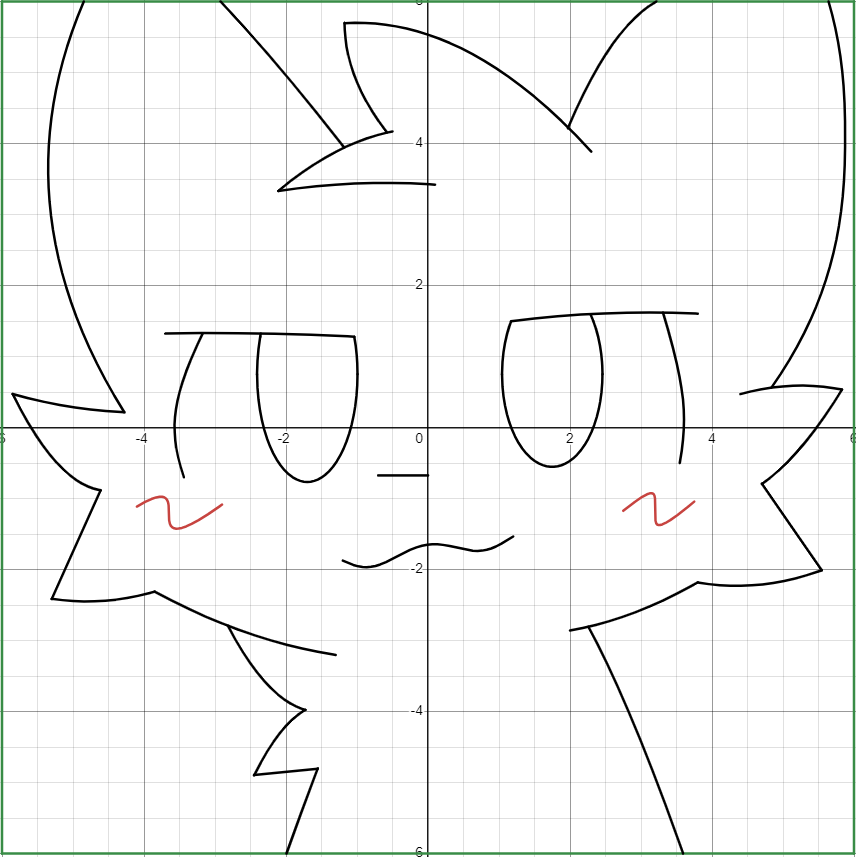
\includegraphics[width=0.75\linewidth]{Year 2/Images/sduijfozunod1.png}
    \caption{You like Fourier series, don't you?}
\end{figure}
As we have just seen, series solutions are a good way to approximate ODE solutions, particular when we expect them to behave similarly to their Taylor series expansions. However we have also covered the minimum radius of convergence which details how these solutions rapidly lose accuracy away from the expansion point. This can be a particular problem for bounded and periodic functions. Mathematically, a function is \(T\)-periodic if for all \(x\):
\[f(x+T)=f(x)\]
In particular we will focus on piecewise continuous and differentiable periodic functions which are functions that can be partitioned into sub-domain intervals in which the function is differentiable. We are allowed jump discontinuities however. In this chapter we study how we can approximate these functions by infinite series of sinusoidal functions. The following integrals will become very helpful:
\[\int^\pi_{-\pi}\sin(mx)\cos(nx)\,\text{d}x=0\]
\[\int^\pi_{-\pi}\sin(nx)\,\text{d}x=\int^\pi_{-\pi}\cos(nx)\,\text{d}x=0\]
\[\int^\pi_{-\pi}\cos(0x)\,\text{d}x=\int^\pi_{-\pi}\,\text{d}x=2\pi\]
\[\int^\pi_{-\pi}\cos(mx)\sin(nx)\,\text{d}x=\begin{cases}
    \pi,& n=m \\
    0, & n\ne m
\end{cases}\]
\[\int^\pi_{-\pi}\sin(mx)\sin(nx)\,\text{d}x=\begin{cases}
    \pi,&n=m \\
    0,&n\ne m
\end{cases}\]
Crucial to demonstrating these facts is knowledge about whether the integrand is even or odd, and what happens when we integrate across a symmetric domain.
\subsection{The Kronecker Delta Function}
We can simplify some of the notation that appears in these integrals by making use of the Kronecker Delta function \(\delta_{nm}\) defined as:
\[\delta_{nm}=\delta_{mn}:=\begin{cases}
    1, & n=m \\
    0, & n\ne m
\end{cases}\]
For example, we could rewrite one of the trigonometric integrals as the following:
\[\int^\pi_{-\pi}\cos(mx)\,\text{d}x=2\pi\delta_{m0}\]
Also note another property of the Kronecker delta - it can "sift" out terms in a sum.
\[\sum^\infty_{n=0}a_n\delta_{nm}=a_0\cdot0+a_1\cdot0+\cdots+a_m\cdot 1=a_m\]
\subsection{Fourier Series of \(2\pi\)-periodic Functions}
For a piecewise continuous and differentiable \(2\pi\)-periodic functions \(f(x)\), the Fourier series of \(f(x)\) is given as:
\[\frac{a_0}{2}+\sum^\infty_{n=1}[a_n\cos(nx)+b_n\sin(nx)]\]
Where the Fourier cosine coefficients \(a_n\) are defined as:
\[a_n=\frac{1}{\pi}\int^\pi_{-\pi}f(x)\cos(nx)\,\text{d}x,\quad n=0,1,2,\dots\]
Whereas the Fourier sine coefficients \(b_n\) are defined as:
\[b_n=\frac{1}{\pi}\int^\pi_{-\pi}f(x)\sin(nx)\,\text{d}x,\quad n=1,2,\dots\]
Notice that the Fourier series does not change when a single point is modified or removed from it's domain of integration. What this means is that any information about piecewise discontinuities of \(f(x)\) is lost.
\subsection{Key Properties of Fourier Series}
\begin{enumerate}
    \item If \(f(x)\) is a combination of sinusoidal functions, then it's Fourier series is identically \(f(x)\), and the coefficients can be read off directly.
    \item Since \(f(x)\) and \(\cos(nx)\) are both \(2\pi\)-periodic, its Fourier coefficient integrals can be evaluated over and domain with full period length:
    \[a_n=\frac{1}{\pi}\int^\pi_{-\pi}f(x)\cos(nx)\,\text{d}x=\frac{1}{\pi}\int^{\theta+2\pi}_\theta f(x)\cos(nx)\,\text{d}x\]
    A similar argument can be made for \(b_n\).
    \item If \(f(x)\) is an odd function, we have \(f(x)\cos(nx)\) is also an odd function and thus \(a_n=0\) over a symmetric domain. Furthermore, since \(f(x)\sin(nx)\) is an even function and so:
    \[b_n=\frac{1}{\pi}\int^\pi_{-\pi}f(x)\sin(nx)\,\text{d}x=\frac{2}{\pi}\int^\pi_0f(x)\sin(nx)\,\text{d}x\]
    \item If \(f(x)\) is an even function, we have \(f(x)\sin(nx)\) is an odd function and thus \(b_n=0\). Furthermore, since \(f(x)\cos(nx)\) is also even, we have that:
    \[a_n=\frac{1}{\pi}\int^\pi_{-\pi}f(x)\cos(nx)\,\text{d}x=\frac{2}{\pi}\int^\pi_{-\pi}f(x)\cos(nx)\,\text{d}x\]
    \item The constant Fourier series term, \(\frac{a_0}{2}\), is always equal to the average value of \(f(x)\) over a full period:
    \[\frac{a_0}{2}=\frac{1}{2\pi}\int^\pi_{-\pi}f(x)\cos(0x)\,\text{d}x=\frac{1}{2\pi}\int^\pi_{-\pi}f(x)\,\text{d}x\]
    \item There are infinitely many functions with the same Fourier series. This is because Fourier integrals lose all information about pointwise discontinuities during the computation. Then for all \(2\pi\)-periodic functions \(f(x)\), the function:
    \[g(x)=\begin{cases}
        f(x) & x\ne a+2n\pi \\
        kf(a) & x=a+2n\pi
    \end{cases}\quad g(x+2\pi)=g(x)\]
\end{enumerate}
\subsubsection{Fourier series of the square wave}
\begin{figure}[H]
    \centering
    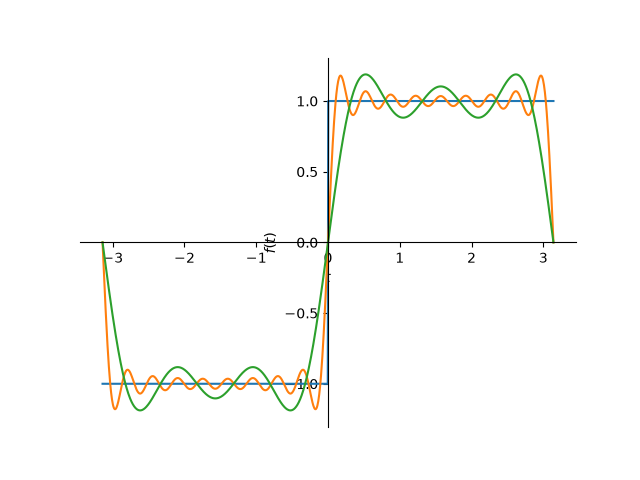
\includegraphics[width=1\linewidth]{Year 2/Images/squarewave.png}
    \caption{A square wave with it's 2-term and 9-term Fourier series}
\end{figure}
In this example, we will find the Fourier series of the square wave function:
\[f(x)=\begin{cases}
    1 & 0<x<\pi \\
    0& \pi<x<2\pi
\end{cases}\quad f(x+2\pi)=f(x)\]
This specific square wave is neither odd nor even so there are no immediate results we can garner from the equations. We will have to compute coefficients. We will also choose to integrate over \([0,2\pi]\) since this interval defines the "base" domain for which \(f(x)\) is defined. Lets start with the cosine coefficients:
\[a_m=\frac{1}{\pi}\int^{2\pi}_0f(x)\cos(nx)\,\text{d}x=\frac{1}{\pi}\int^\pi_0\cos(nx)\,\text{d}x=\frac{sin(nx)}{n\pi}\bigr|^\pi_0=0\]
Note that we only have this when \(n\ne 0\) otherwise we would be evaluating a division by 0. Because of this we need to calculate \(a_0\) separately.
\[a_0=\frac{1}{\pi}\int^{2\pi}_0f(x)\cos(0x)\,\text{d}x=\frac{1}{\pi}\int^{2\pi}_0f(x)\,\text{d}x=1\]
Now we need to compute the Fourier since coefficients:
\[b_n=\frac{1}{\pi}\int^{2\pi}_0f(x)\sin(nx)\,\text{d}x=\frac{1}{\pi}\int^\pi_0\sin(nx)\,\text{d}x=\frac{-\cos(n\pi)}{n\pi}\bigr|^\pi_0\]
\[\frac{-\cos(n\pi)}{n\pi}\bigr|^\pi_0=\frac{1-\cos(n\pi)}{n\pi}=\frac{1-(-1)^n}{n\pi}\]
Note that this last simplification step is very commonly done when dealing with Fourier series. Putting this altogether, we can see that the Fourier series for our example square wave is:
\[f(x)\sim \frac{1}{2}+\sum^\infty_{n=1}\frac{[1-(-1)^n]\sin(nx)}{n\pi}\]
\subsection{Fourier Convergence Theorem}
As we have already seen, the Fourier series of a function loses all information about piecewise discontinuities. Furthermore, piecewise discontinuities do not change the value of the resulting integral and so are not accurately captured in the first place. Nevertheless it is still possible to determine the behaviour of a Fourier series at a jump discontinuity. This is known as the Fourier convergence theorem: For a piecewise continuous and differentiable \(2\pi\)-periodic function \(f(x)\), suppose that it's \(N^{th}\) partial Fourier series \(S_N(x)\) is given as:
\[S_N(x)=\frac{a_0}{2}+\sum^N_{n=1}[a_n\cos(nx)+b_n\sin(nx)]\]
The Fourier convergence theorem states that:
\[\lim_{N\to\infty}S_N(x)=\frac{f(x+)+f(x-)}{2},\quad \forall x\]
Where \(f(x+)\) and \(f(x-)\) denote the one-sided limits of \(f(z)\) at \(z=x\):
\begin{align*}
    f(x+):=\lim_{z\to x^+}f(z) && f(x-):=\lim_{z\to x^-}f(z)
\end{align*}
In words, the Fourier series of \(f(x)\) converges to exactly \(f(x)\) for all points that are continuous and converges to the average of it's one-sided limits at jump discontinuities. We can use the symbol \(\sim\) to denote equality up to discontinuity.
\[f(x)\sim\frac{a_0}{2}+\sum^\infty_{n=1}[a_n\cos(nx)+b_n\sin(nx)]\]
\begin{figure}[H]
    \centering
    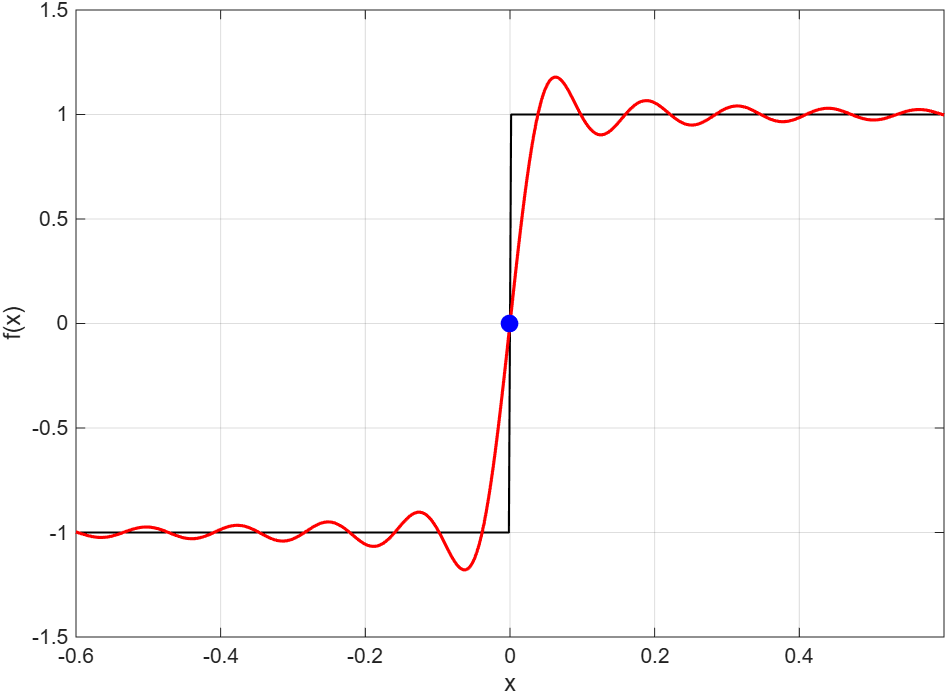
\includegraphics[width=0.75\linewidth]{Year 2/Images/FCT_demo.png}
    \caption{The Fourier series will converge to the midpoint of the discontinuity}
\end{figure}
\subsubsection{Evaluating infinite series using FCT}
Consider the square wave we looked at earlier. We wish to use the FCT to determine the value of the infinite sum:
\[S=\sum^\infty_{m=0}\frac{(-1)^m}{2m+1}\]
At first glance, this sum bears no resemblance to our Fourier series for the square wave. However consider that the Fourier series of the square wave is continuous at \(x=\frac{\pi}{2}\) with \(f(\frac{\pi}{2})=1\). Also notice that not all values of \(n\) contribute any terms to our Fourier series of \(f(x)\). In particular:
\[1-(-1)^n=\begin{cases}
    0 & n\text{ even} \\
    2& n\text{ odd}
\end{cases}\]
Then we only need sum of over odd values of \(n\) and now we should notice a familiar series:
\[1=\frac{1}{2}+\sum^\infty_{m=0}\frac{2}{(2m+1)\pi}\sin\left(\frac{(2m+1)\pi}{2}\right)=\frac{1}{2}+\frac{2}{\pi}\sum^\infty_{m=0}\frac{(-1)^m}{2m+1}\]
To see that last simplification step, consider the bounds of the \(\sin\) term and what values it can take for \(m\in\mathbb{Z}\). Therefore:
\[1=\frac{1}{2}+\frac{2S}{\pi}\implies S=\frac{\pi}{4}\]
\subsection{Continuous vs Piecewise Continuous Functions}
A natural question would be is it possible to identify when a function has piecewise discontinuities from its Fourier series. The answer is yes! Consider the triangle wave function as an example:
\[g(x)=\begin{cases}
    \frac{\pi}{2}+x& -\pi\leq x<0 \\
    \frac{\pi}{2}-x & 0\leq x< \pi
\end{cases},\quad g(x+2\pi )=g(x)\]
We can see by inspection that the function \(g(x)\) is continuous for all \(x\). It is also even, which lets us know that all \(\sin\) terms in the Fourier series will be \(0\):
\[b_n=0\]
We can work through the integrals and eventually find that the Fourier series of \(g(x)\) is given by:
\[g(x)=\frac{2}{\pi}\sum^\infty_{n=1}\frac{[1-(-1)^n]\cos(nx)}{n^2}\]
Now notice the coefficients \(a_n\) and how quickly they decay. In the case of the triangle wave, the \(a_n\) coefficients decay proportional to \(n^{-2}\). This is certainly faster than that of the square wave which decayed proportional to \(n^{-1}\). This has a dramatic effect on how quickly the Fourier series converges to the function. Decay rates are key characteristics of Fourier series that indicate if a Fourier series represents a function that is continuous everywhere or piecewise continuous. The TLDR of this is that if the decay rate of either Fourier coefficients is proportional to \(n^{-1}\), then the function \(f(x)\) contains piecewise discontinuities.
\subsection{Gibbs Phenomenon}
As we just mentioned, the decay rate of the Fourier coefficients is critical to describing the nature of the original function. There are some other peculiarities that arise at points of discontinuity due to bounded sinusoidal functions being multiplied with coefficients that produce conditionally convergent or divergent infinite series. Essentially the more terms that we have, the more they really want to diverge at points of discontinuity but can't because they are bounded. What this leads to is known as Gibbs Phenomenon and is when the Fourier series cannot accurately approximate a function in the lead up to a jump discontinuity and is has a guaranteed overshoot/undershoot amount.
\begin{figure}
    \centering
    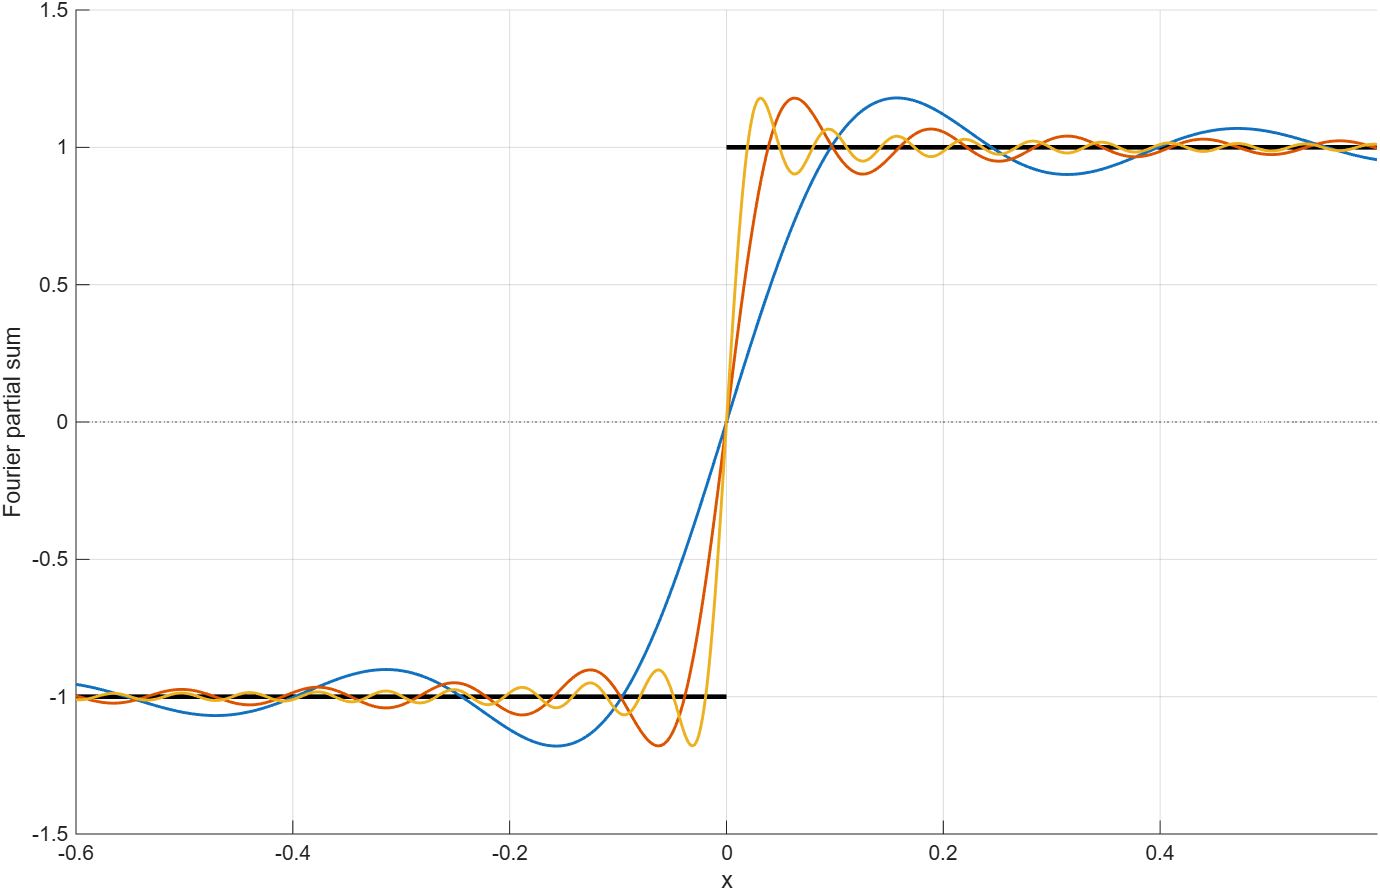
\includegraphics[width=1\linewidth]{Year 2/Images/Gibbs.png}
    \caption{Gibbs Phenomenon doesn't disappear with more terms.}
\end{figure}
In signal processing, these overshoots and undershoots are sometimes referred to as "chirping". Notably Gibbs Phenomenon does not vanish as more and more terms of the Fourier series are added.
\subsection{Fourier Series of \(2L\)-periodic Functions}
Not all functions are going to have a period of \(2\pi\), so we present the same results for periodic functions with any given finite period \(T=2L\). Fortunately we can construct the linear map \(y=\frac{\pi x}{L}\) which maps \([-L,L]\) to \([-\pi,\pi]\) and from there we can use all of the same results. These are stated on the formula sheet:
\[f(x)\sim \frac{a_0}{2}+\sum^\infty_{n=0}\left[a_n\cos\left(\frac{n\pi x}{L}\right)+b_n\sin\left(\frac{n\pi x}{L}\right)\right]\]
Where the coefficients are defined as:
\[a_n=\frac{1}{L}\int^L_{-L}f(x)\cos\left(\frac{n\pi x}{L}\right)\,\text{d}x,\quad n\geq 0\]
\[b_n=\frac{1}{L}\int^L_{-L}f(x)\sin\left(\frac{n\pi x}{L}\right)\,\text{d}x,\quad n\geq 1\]
Notice that we retrieve the original definition by setting \(L=\pi\). It is very important to remember that \(L\) is the half-period of the function and not the entire period. If in doubt, think back to how \(\pi\) behaves for the \(2\pi\)-periodic functions.
\subsubsection{Example of a non-standard period function}
In this example we will consider the Fourier series of the "sawtooth" wave defined as:
\[h(x)=x,\quad x\in(-1,1),\quad h(x+2)=h(x)\]
Notice that the period is \(2\) which implies the half period \(L=1\). Additionally notice that the function is odd so \(a_n=0\). We compute the sine coefficients:
\[b_n=\frac{1}{1}\int^{1}_{-1}h(x)\sin(n\pi x)\,\text{d}x=2\int^1_0x\sin( n\pi x)\,\text{d}x\]
\[b_n=\frac{2(-1)^{n+1}}{n\pi}\]
Then the Fourier series of the sawtooth function is:
\[h(x)\sim\frac{2}{\pi}\sum^\infty_{n=1}\frac{(-1)^{n+1}}{n}\sin(n\pi x)\]
\begin{figure}[H]
    \centering
    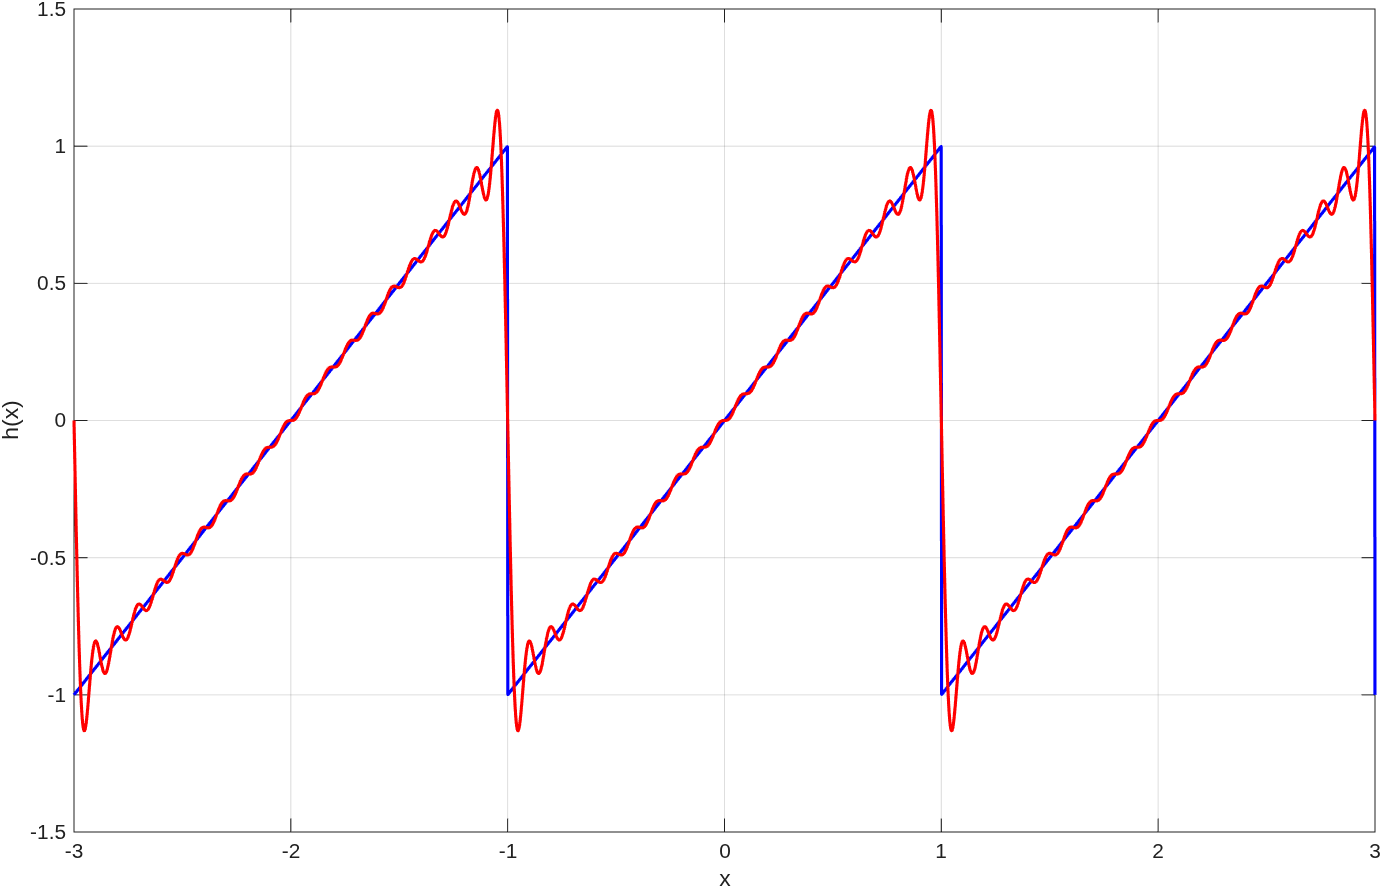
\includegraphics[width=0.75\linewidth]{Year 2/Images/sawwtooth.png}
    \caption{Sawtooth function and its Fourier series.}
\end{figure}
\subsection{Period Extensions of Non-periodic Functions}
In this section, we consider ways to extend a non-periodic function into a periodic one. This might seem redundant at this stage but is crucial for our later work. Consider a function \(f(x)\) that is defined on \((0,L)\) noting that our endpoints are not included. There are 3 natural extensions to turn a \(f(x)\) into a periodic function.
\subsubsection{Identity reflection}
In this case we extend the function by just repeating it over an extended domain:
\[\tilde{f}(x)=f(x);\; x\in(0,L),\quad \tilde{f}(x+L)=\tilde{f}(x)\]
This formulation is very important because it allows us to find the Fourier coefficients on any domain of width \(L\), so trivially we can take \((0,L)\) - which is the original domain of the function - hence we can extract information from only the non-periodic segment since \(\tilde{f}(x)=f(x)\) on this domain.
\subsubsection{Odd periodic extension}
In this case we define the periodically-extended function \(f_o(x)\) as:
\[f_o(x)=\begin{cases}
    f(x)&x\in(0,L) \\
    -f(-x) & x\in(-L,0)
\end{cases},\quad f_o(x+2L)=f_o(x)\]
Notice we now have an odd function defined in the domain \((-L,L)\). This new function is periodic. Once again we can now compute Fourier coefficients. In this case we have \(a_n=0\):
\[f_o(x)\sim\sum^\infty_{n=1}b_n\sin\left(\frac{n\pi x}{L}\right)\]
We have \(f_o(x)=f(x)\) on the domain \((0,L)\).
\subsubsection{Even periodic extension}
Define the even periodically-extended function \(f_e(x)\) as:
\[f_e(x)=\begin{cases}
    f(x)&x\in(0,L)\\
    f(-x) & x\in(-L,0)
\end{cases},\quad f_e(x+2L)=f_e(x)\]
Since \(f_e(x)\) is by definition an even function, we have \(b_n=0\) and thus the Fourier series is:
\[f_e(x)\sim\frac{a_0}{2}+\sum^\infty_{n=1}a_n\cos\left(\frac{n\pi x}{L}\right)\]
Notice again \(f_e(x)=f(x)\) only on \((0,L)\)
\clearpage
\section{Introduction to PDEs}
\end{document}